% 原脑影像/全部连边与颜色保留；中文标签在原PDF文字层对应位置覆盖。
\begin{figure}[htbp]
\centering
\begin{tikzpicture}[x=1cm,y=1cm]
\node[anchor=south west,inner sep=0] at (0,0) {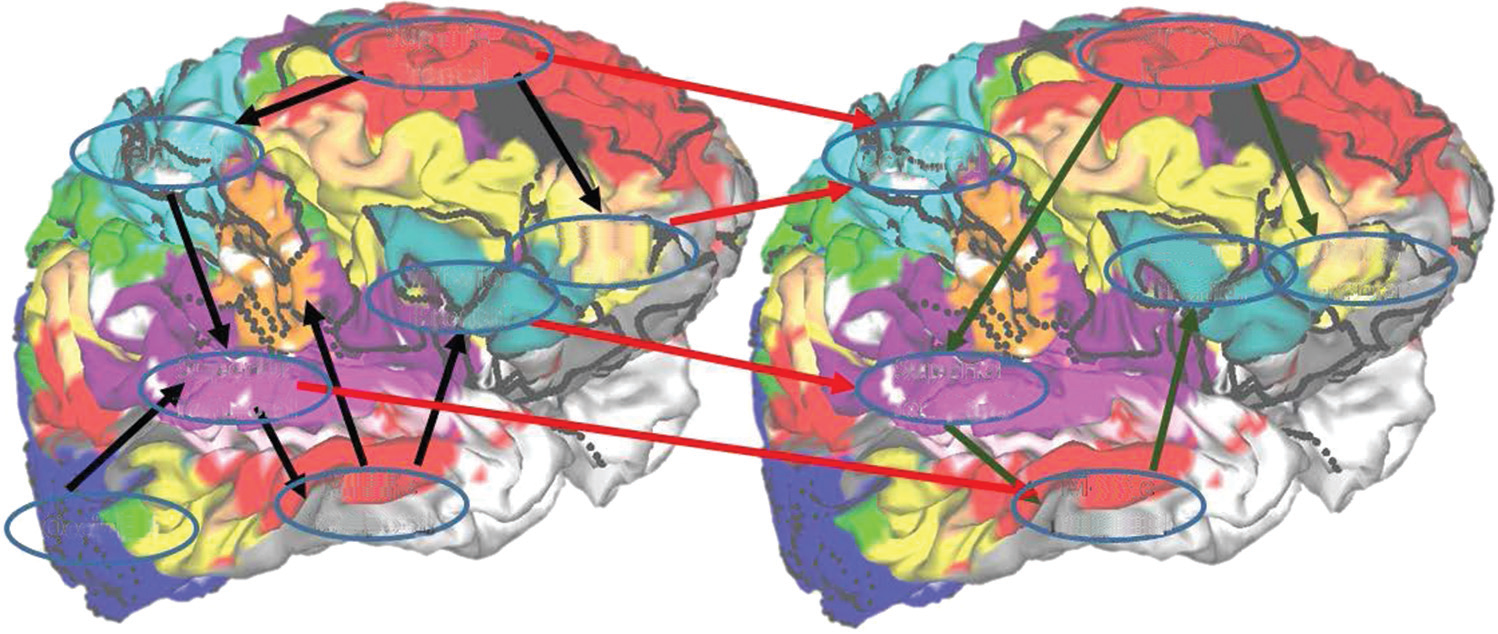
\includegraphics[width=14cm]{figures/ch06_figure15_data.png}};
\node[font=\scriptsize,fill=white,fill opacity=.88,text opacity=1,inner sep=1pt] at (4.1402,5.4766) {额上区};
\node[font=\scriptsize,fill=white,fill opacity=.88,text opacity=1,inner sep=1pt] at (1.5888,4.5234) {中央区};
\node[font=\scriptsize,fill=white,fill opacity=.88,text opacity=1,inner sep=1pt] at (5.9346,3.6355) {眶额区};
\node[font=\scriptsize,fill=white,fill opacity=.88,text opacity=1,inner sep=1pt] at (4.3645,3.1589) {额下区};
\node[font=\scriptsize,fill=white,fill opacity=.88,text opacity=1,inner sep=1pt] at (2.2243,2.3084) {颞上区};
\node[font=\scriptsize,fill=white,fill opacity=.88,text opacity=1,inner sep=1pt] at (3.4860,1.1495) {颞中区};
\node[font=\scriptsize,fill=white,fill opacity=.88,text opacity=1,inner sep=1pt] at (0.9439,1.0093) {枕区};
\node[font=\scriptsize,fill=white,fill opacity=.88,text opacity=1,inner sep=1pt] at (11.1869,5.4579) {额上区};
\node[font=\scriptsize,fill=white,fill opacity=.88,text opacity=1,inner sep=1pt] at (8.6449,4.4486) {中央区};
\node[font=\scriptsize,fill=white,fill opacity=.88,text opacity=1,inner sep=1pt] at (12.9439,3.4953) {眶额区};
\node[font=\scriptsize,fill=white,fill opacity=.88,text opacity=1,inner sep=1pt] at (11.1589,3.3178) {额下区};
\node[font=\scriptsize,fill=white,fill opacity=.88,text opacity=1,inner sep=1pt] at (8.9346,2.3178) {颞上区};
\node[font=\scriptsize,fill=white,fill opacity=.88,text opacity=1,inner sep=1pt] at (10.3738,1.1495) {颞中区};
\node at (3.5,-.35) {$T_0$};\node at (10.5,-.35) {$T_1$};
\end{tikzpicture}
\origfig{15}{fMRI 的有效连接图。}
\end{figure}
